%
% Capítulo 3
%
\chapter{Solução Proposta} \label{cap3}

Neste capítulo pretende-se dar ênfase à solução implementada para resolver o problema apresentado no capítulo \ref{cap2}. Este capítulo está divido nas seguintes secções, Modelo de Dados na secção \ref{sec31}, \acrlong{bd} na secção \ref{sec32}, Acesso a Dados na secção \ref{sec33} e Lógica de Negócio na secção \ref{sec34}.

\begin{figure}[H]
	\centering
	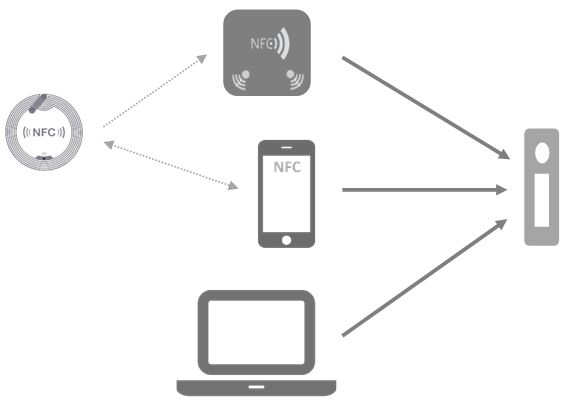
\includegraphics[width=12cm, scale=1]{./figures/project_structures.png}
	\caption{Estrutura do Projeto}
	\label{project-structure}
\end{figure}

\begin{center}
	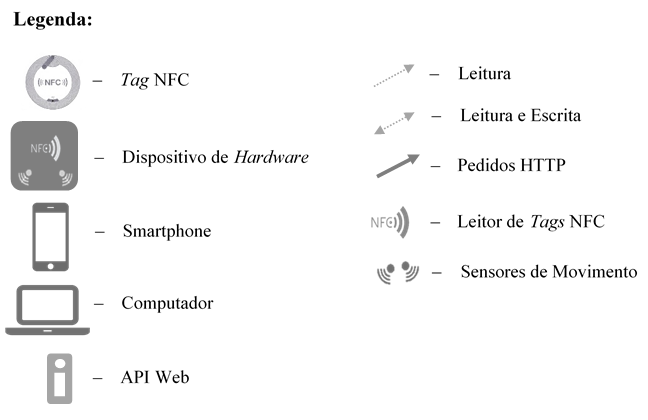
\includegraphics[width=12cm, scale=1]{./figures/project_structures_caption.png}
\end{center}

Com a Figura \ref{project-structure} pretende-se não só apresentar os principais componentes do projeto, bem como demonstrar de forma breve a relação dos mesmos. É de destacar que uma \textit{tag} pode ser lida por um dispositivo de \textit{hardware} munido de um leitor de \textit{tags}. Um \textit{smartphone} equipado com tecnologia \acrshort{nfc} pode escrever na \textit{tag} \acrshort{nfc}, tal é necessário para identificar produtos avulsos presentes num sistema de arrumação. Tanto o dispositivo de \textit{hardware} como as aplicações, móvel e \textit{web}, comunicam com a \gls{api-web}.\\

O projeto é composto por 2 blocos principais, que se relacionam. A Figura \ref{project-architecture} representa esses blocos. 

\begin{figure}[H]
	\centering
	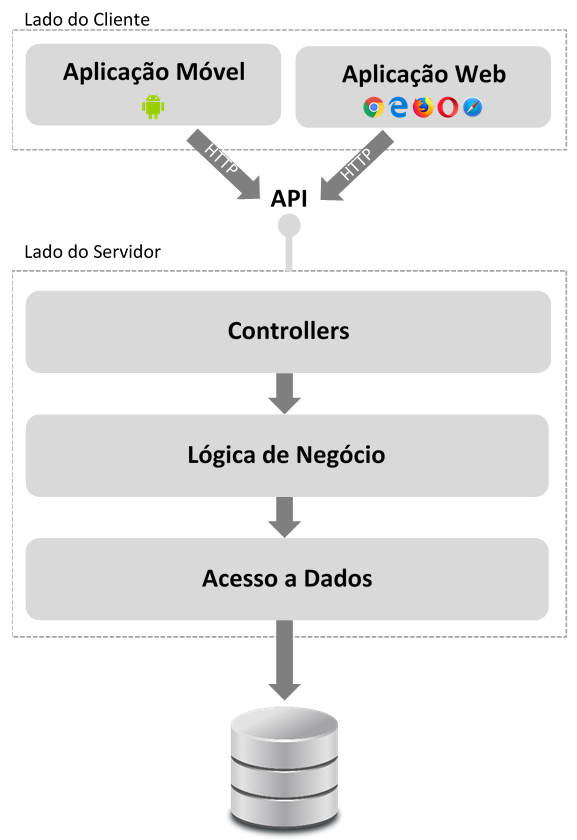
\includegraphics[height=9cm, scale=1]{./figures/project_architecture.png}
	\caption{Arquitetura do Projeto}
	\label{project-architecture}
\end{figure}

O lado do servidor incluí quatro camadas e expõe uma \gls{api-web}. A camada da \acrfull{bd} é realizada com o \acrfull{sgbd} \textit{PostgreSQL}. A \acrfull{dal} é responsável pelas leituras e escritas à \acrshort{bd}. Esta camada é produzida com a linguagem de programação \textit{Java}, com a \acrfull{jpa}. A \acrfull{bll} é responsável pela gestão dos dados obtidos da \acrshort{bd} ou dos \textit{controllers}. A implementação desta camada recorreu à mesma ferramenta que foi usada na \acrshort{dal}. Os \textit{controllers} foram desenvolvidos em \textit{Java} com a \textit{framework} da \textit{Spring}, chamada de \textit{Spring Boot}. A \gls{api-web} disponibiliza recursos em diferentes \textit{hypermedia}.

Do lado do cliente existem dois modos de interação, por uma aplicação móvel e outra por uma aplicação web. A aplicação móvel disponível para a plataforma \textit{Android}, desenvolvida em linguagem \textit{Kotlin}. A aplicação web é disponibilizada para a maioria dos browsers, implementada utilizando a linguagem \textit{JavaScript}, com o auxilio da \textit{framework Express}.

%
% Modelo de Dados
%
\section{Modelo de Dados}\label{sec31}



% Modelo EA
\subsection{Modelo Entidade-Associação}\label{subsec311}

\begin{figure}[H]
	\hspace*{-2,5cm}
	\centering
	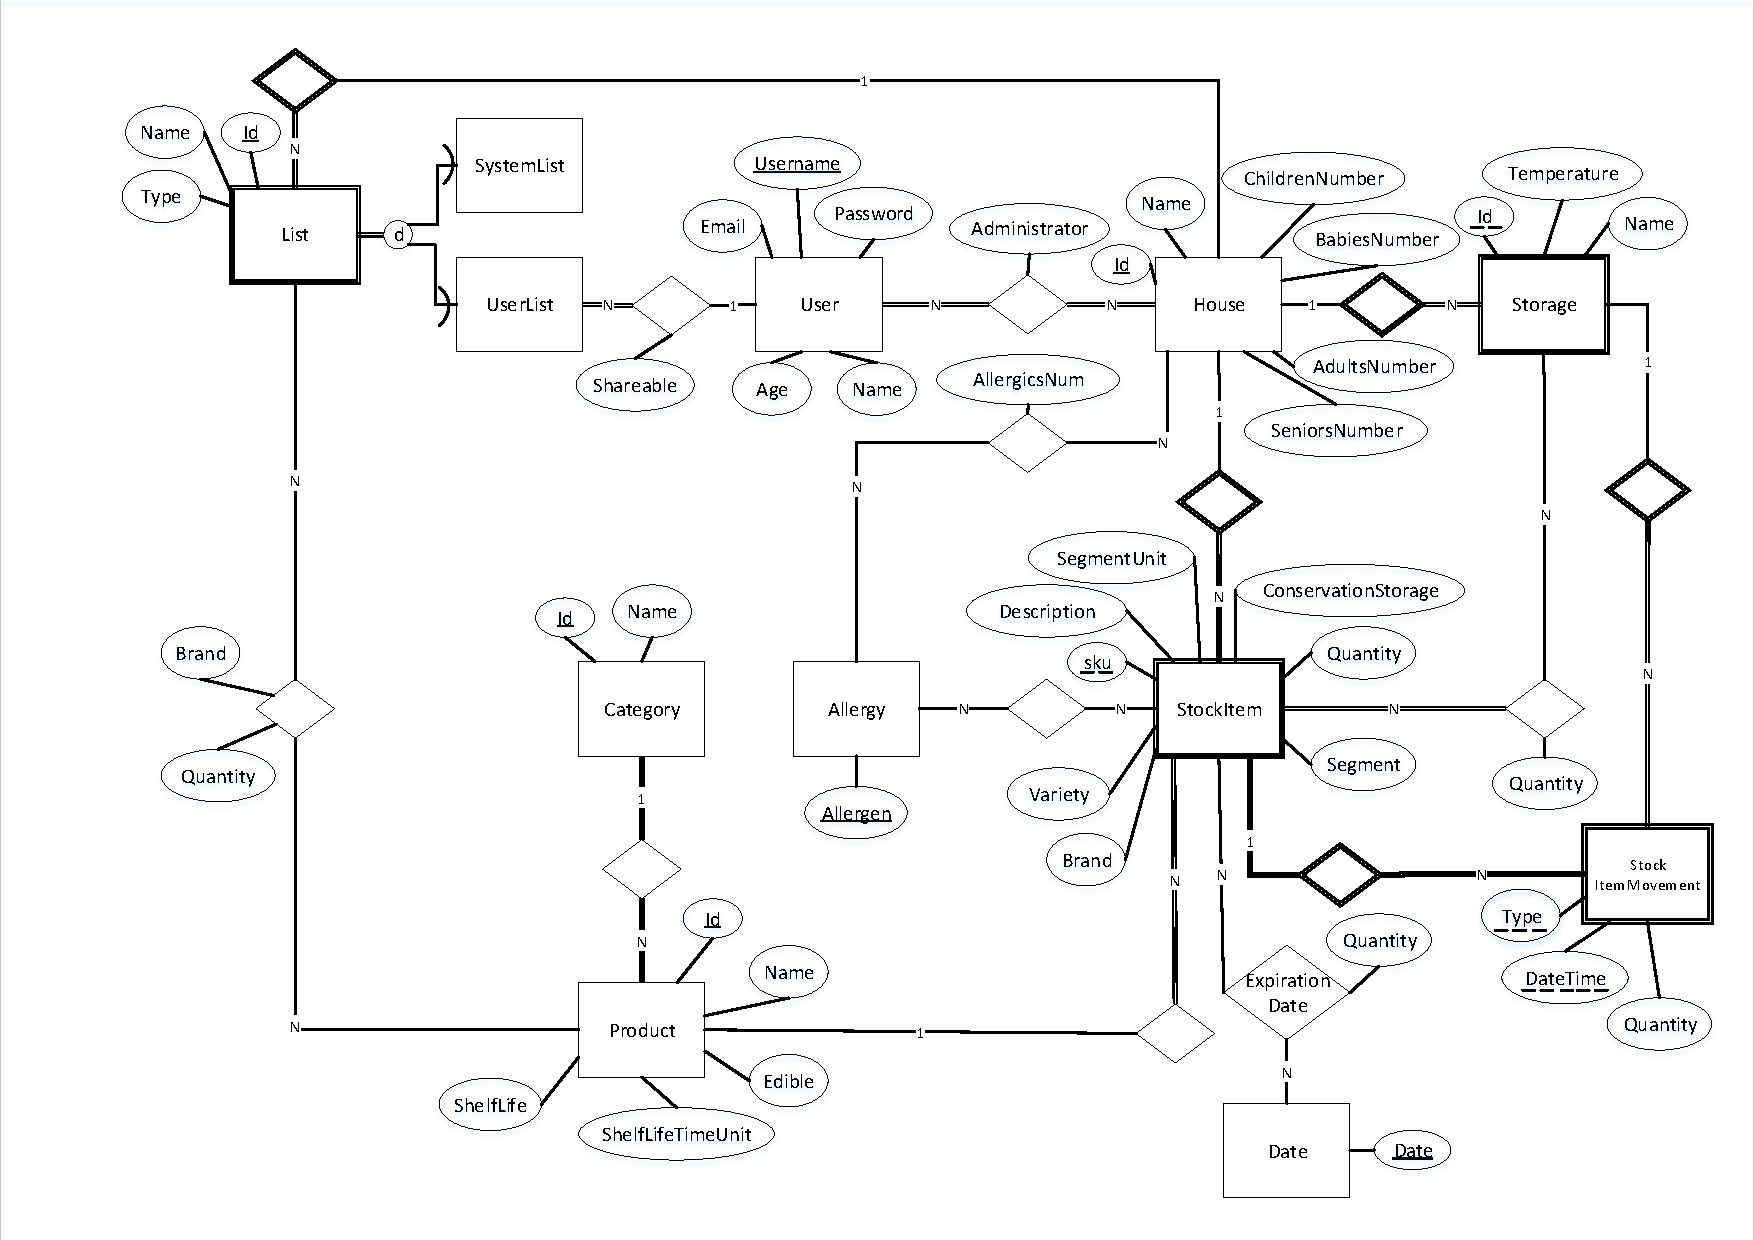
\includegraphics[width=20cm,height=15cm,scale=1]{./files/EA.pdf}
	\caption{Modelo Entidade-Associação}
	\label{modelo-ea}
\end{figure}

% Modelo Relacional
\subsection{Modelo Relacional}\label{subsec312}

{\parindent 0pt
	\begin{description}
		\item House(house\_id, house\_name, house\_babiesNumber, house\_childrenNumber, house\_adultsNumber, house\_seniorsNumber) \newline
		\acrshort{cp}: (house\_id) 
		
		\item User(user\_username, user\_email, user\_age, user\_name, user\_password) \newline
		\acrshort{cp}: (user\_username)  \newline
		\acrshort{occ}: (user\_email)
		
		\item Allergy(allergy\_allergen) \newline
		\acrshort{cp}: (allergy\_allergen) 
		
		\item Recipe(recipe\_id, recipe\_name, recipe\_instructions, recipe\_difficulty, recipe\_time, recipe\_servings, recipe\_cuisine, recipe\_dishType, recipe\_type) \newline
		\acrshort{cp}: (recipe\_id) 
		
		\item SystemRecipe(recipe\_id) \newline
		\acrshort{cp}: (recipe\_id) \newline
		\acrshort{ce}: \{(recipe\_id) ref Recipe\}
		
		\item UserRecipe(recipe\_id, user\_username) \newline
		\acrshort{cp}: (recipe\_id) \newline
		\acrshort{ce}: \{(recipe\_id) ref Recipe, (user\_username) ref User\}
		
		\item SharedRecipe(recipe\_id, user\_username) \newline
		\acrshort{cp}:(recipe\_id, user\_username) \newline
		\acrshort{ce}: \{(recipe\_id) ref UserRecipe, (user\_username) ref User\}
		
		\item List(house\_id, list\_id, list\_name, list\_type) \newline
		\acrshort{cp}: (house\_id, list\_id) \newline
		\acrshort{ce}: \{(house\_id) ref House\}
		
		\item SystemList(house\_id, list\_id)
		\newline
		\acrshort{cp}: (house\_id, list\_id) \newline
		\acrshort{ce}: \{(house\_id, list\_id) ref List\}
		
		\item UserList(house\_id, list\_id, user\_username, list\_shareable)
		\newline
		\acrshort{cp}: (house\_id, list\_id) \newline
		\acrshort{ce}: \{(house\_id, list\_id) ref List, (user\_username) ref User\}
		
		\item Category(category\_id, category\_name)
		\newline
		\acrshort{cp}: (category\_id) \newline
		\acrshort{occ}: (category\_name)
		
		\item Product(category\_id, product\_id, product\_name, product\_edible, product\_shelfLife, \newline product\_shelfLifeTimeUnit) \newline
		\acrshort{cp}: (category\_id, product\_id) \newline
		\acrshort{ce}: \{(category\_id) ref Category\}
		
		\item StockItem(house\_id, stockItem\_sku, category\_id, product\_id, stockItem\_brand, stockItem\_segment, stockItem\_variety, stockItem\_quantity, stockItem\_segmentUnit, stockItem\_description, stockItem\_conservationStorage) \newline
		\acrshort{cp}: (house\_id, stockItem\_sku) \newline
		\acrshort{occ}: (house\_id, category\_id, product\_id, stockItem\_brand, stockItem\_segment, \newline stockItem\_variety) \newline
		\acrshort{ce}: \{(house\_id) ref House, (category\_id, product\_id) ref Product\}
		
		\item Ingredient(recipe\_id, category\_id, product\_id, ingredient\_quantity, ingredient\_quantityUnit) \newline
		\acrshort{cp}: (recipe\_id, category\_id, product\_id) \newline
		\acrshort{ce}: \{(recipe\_id) ref Recipe, (category\_id, product\_id) ref Product\}
		
		\item Storage(house\_id, storage\_id, storage\_name, storage\_temperature)  \newline
		\acrshort{cp}:(house\_id, storage\_id) \newline
		\acrshort{ce}: \{(house\_id) ref House\}
		
		\item UserHouse(house\_id, user\_username, userHouse\_administrator) \newline
		\acrshort{cp}: (house\_id, user\_username) \newline
		\acrshort{ce}: \{(house\_id) ref House, (user\_username) ref User\}
		
		\item StockItemStorage(house\_id, stockItem\_sku, storage\_id, stockItemStorage\_quantity) \newline
		\acrshort{cp}: (house\_id, stockItem\_sku, storage\_id) \newline
		\acrshort{ce}: \{(house\_id, stockItem\_sku) ref StockItem, (house\_id, storage\_id) ref Storage\}
		
		\item StockItemMovement(house\_id, stockItem\_sku, storage\_id, stockItemMovement\_type, \newline stockItemMovement\_dateTime) \newline
		\acrshort{cp}: (house\_id, stockItem\_sku, storage\_id, stockItemMovement\_type, \newline stockItemMovement\_dateTime) \newline
		\acrshort{ce}: \{(house\_id, stockItem\_sku) ref StockItem, (house\_id, storage\_id) ref Storage\}
		
		\item HouseAllergy(house\_id, allergy\_allergen, houseAllergy\_alergicsNum) \newline
		\acrshort{cp}: (house\_id, allergy\_allergen) \newline
		\acrshort{ce}: \{(house\_id) ref House, (allergy\_allergen) ref Allergy\}
		
		\item ListProduct(house\_id, list\_id, category\_id, product\_id, listProduct\_brand, listProduct\_quantity) \newline
		\acrshort{cp}: (house\_id, list\_id, category\_id, product\_id) \newline
		\acrshort{ce}: \{(house\_id, list\_id) ref List, (category\_id, product\_id) ref Product\}
		
		\item StockItemAllergy(house\_id, stockItem\_sku, allergy\_allergen) \newline
		\acrshort{cp}: (house\_id, stockItem\_sku, allergy\_allergen) \newline
		\acrshort{ce}: \{(house\_id, stockItem\_sku) ref StockItem, (allergy\_allergen) ref Allergy\}
		
		\item Date(date\_date) \newline
		\acrshort{cp}: (date\_date)
		
		\item ExpirationDate(house\_id, stockItem\_sku, date\_date) \newline
		\acrshort{cp}: (house\_id, stockItem\_sku, date\_date) \newline
		\acrshort{ce}: \{(house\_id, stockItem\_sku) ref StockItem, (date\_date) ref Date\}
	\end{description}	
}


\subsubsection{Restrições de Integridade}
\begin{description}
	\item RI1: house\_id é auto-incrementado;
	\item RI2: house\_name é uma cadeia de caracteres obrigatória de comprimento máximo 35, pode incluir letras, números, pontos finais e underscores;
	\item RI3: house\_characteristics é um objeto \acrshort{json} obrigatório;
	\item RI4: user\_username é uma cadeia de caracteres obrigatória de comprimento máximo 30, pode incluir letras, números, pontos finais e underscores;
	\item RI5: user\_email é uma cadeia de caracteres obrigatória de comprimento máximo 254, pode incluir letras, números, pontos finais, underscores e um arroba;
	\item RI6: user\_age é um número inteiro obrigatório contido no intervalo [0, 150];
	\item RI7: user\_name é uma cadeia de caracteres obrigatória de comprimento máximo 70, sendo apenas composta por letras;
	\item RI8: user\_password é uma cadeia de caracteres obrigatória de comprimento máximo 50, pode incluir letras, números e caracteres especiais;
	\item RI9: allergy\_allergen é uma cadeia de caracteres obrigatória de comprimento máximo 75;
	\item RI10: recipe\_id é auto-incrementado;
	\item RI11: recipe\_name é uma cadeia de caracteres obrigatória de comprimento máximo 35, pode incluir letras, números, pontos finais e underscores;
	\item RI12: recipe\_difficulty é opcional e pode tomar um dos valores [‘easy’, ‘average’, ‘difficult’];
	\item RI13: recipe\_time é um número inteiro opcional superior a 0;
	\item RI14: recipe\_servings é um número inteiro opcional superior a 0;
	\item RI15: recipe\_cuisine é uma cadeia de caracteres opcional de comprimento máximo 35;
	\item RI16: recipe\_dishType é uma cadeia de caracteres opcional de comprimento máximo 35;
	\item RI17: recipe\_type é obrigatório e tem de tomar um dos valores [‘system, ‘user];
	\item RI18: list\_id é único dentro da casa;
	\item RI19: list\_name é uma cadeia de caracteres obrigatória de comprimento máximo 35, pode incluir letras, números, pontos e underscores;
	\item RI20: list\_type é obrigatório e tem de tomar um dos valores [‘system, ‘user];
	\item RI21: category\_id é auto-incrementado;
	\item RI22: category\_name é uma cadeia de caracteres obrigatória de comprimento máximo 35, sendo apenas composta por letras;
	\item RI23: product\_id é único dentro da categoria;
	\item RI24: product\_name é uma cadeia de caracteres obrigatória de comprimento máximo 35, sendo apenas composta por letras;
	\item RI25: product\_edible é obrigatório e tem de tomar um dos valores ['true', 'false'];
	\item RI26: product\_shelfLife é um número inteiro obrigatório superior a 0;
	\item RI27: product\_shelfLifeTimeUnit é obrigatório e tem de tomar um dos valores [‘day’, ‘week’, ‘month’, ‘year’];
	\item RI28: stockItem\_sku é uma cadeia de caracteres obrigatória de comprimento máximo 128, gerada pela composição de category\_id, product\_id, stockItem\_brand, stockItem\_segment e stockItem\_variety;
	\item RI29: stockItem\_brand é uma cadeia de caracteres obrigatória de comprimento máximo 35;
	\item RI30: stockItem\_segment é uma cadeia de caracteres obrigatória de comprimento máximo 35;
	\item RI31: stockItem\_variety é uma cadeia de caracteres obrigatória de comprimento máximo 35;
	\item RI32: stockItem\_quantity é um número inteiro obrigatório superior a 0;
	\item RI33: stockItem\_segmentUnit é obrigatório e tem de tomar um dos valores [‘kg’, ‘dag’, ‘hg’, ‘g’, ‘dg’, ‘cg’, ‘mg’, ‘kl’, ‘hl’, ‘dal’, ‘l’, ‘dl’, ‘cl’, ‘ml’, ‘oz’, ‘lb’, ‘pt’, ‘fl oz’, ‘units’];
	\item RI34: stockItem\_conservationStorage é uma cadeia de caracteres obrigatório de comprimento máximo 128;
	\item RI35: ingredient\_quantity é um número inteiro obrigatório superior a 0;
	\item RI36: ingredient\_quantityUnit é obrigatório e tem de tomar um dos valores [‘kg’, ‘dag’, ‘hg’, ‘g’, ‘dg’, ‘cg’, ‘mg’, ‘kl’, ‘hl’, ‘dal’, ‘l’, ‘dl’, ‘cl’, ‘ml’, ‘oz’, ‘lb’, ‘pt’, ‘fl oz’, ‘units’];
	\item RI37: storage\_id é único dentro da casa;
	\item RI38: storage\_name é uma cadeia de caracteres de comprimento máximo 35;
\end{description}

% Domínio dos Atributos
\subsection{Domínio dos Atributos}\label{subsec313}
\raggedbottom
% House
\begin{table} [H]
	\centering
	\caption{Domínio dos Atributos da Entidade House.} \vspace{2mm}
	\label{tab-dominio-atributos-house}
	\resizebox{\textwidth}{!}{%
		\begin{tabular}{|c|c|c|c|c|c|}
			\hline
			\textbf{Entidade} & \textbf{Atributo} & \textbf{Domínio} & \textbf{Tipo Variável (PostgreSQL)} & \textbf{Restrições} & \textbf{Nullable}\\ \hline
			\multirow{6}{*}{House} & house\_id & Número inteiro auto-incrementado & bigserial & - & não\\ \cline{2-6}
			& house\_name & Cadeia de caracteres de comprimento variável & character varying(35) & até 35 caracteres & não\\ \cline{2-6}
			& house\_characteristics & Objeto \acrshort{json} & json & - & não\\ \hline
		\end{tabular}
	}
\end{table}

% User
\begin{table} [H]
	\centering
	\caption{Domínio dos Atributos da Entidade User.} \vspace{2mm}
	\label{tab-dominio-atributos-user}
	\resizebox{\textwidth}{!}{%
		\begin{tabular}{|c|c|C{2.5cm}|C{2.7cm}|C{3.6cm}|C{2.3cm}|}
			\hline
			\textbf{Entidade} & \textbf{Atributo} & \textbf{Domínio} & \textbf{Tipo Variável (PostgreSQL)} & \textbf{Restrições} & \textbf{Nullable}\\ \hline
			\multirow{5}{*}{User} & user\_username & Cadeia de caracteres de comprimento variável & character varying(30) & até 30 caracteres & não\\ \cline{2-6}
			& user\_email & Cadeia de caracteres de comprimento variável & character varying(254) & até 254 caracteres & não\\ \cline{2-6}
			& user\_age & Número inteiro & smallint & user\_age in [0, 150] & não\\ \cline{2-6}
			& user\_name & Cadeia de caracteres de comprimento variável & character varying(70) & até 70 caracteres & não\\ \cline{2-6}
			& user\_password & Cadeia de caracteres de comprimento variável & character varying(50) & até 50 caracteres & não\\ \hline
		\end{tabular}
	}
\end{table}

% Allergy
\begin{table} [H]
	\centering
	\caption{Domínio dos Atributos da Entidade Allergy.} \vspace{2mm}
	\label{tab-dominio-atributos-allergy}
	\resizebox{\textwidth}{!}{%
		\begin{tabular}{|c|c|C{2.5cm}|C{2.7cm}|C{3.6cm}|C{2.3cm}|}
			\hline
			\textbf{Entidade} & \textbf{Atributo} & \textbf{Domínio} & \textbf{Tipo Variável (PostgreSQL)} & \textbf{Restrições} & \textbf{Nullable}\\ \hline
			{Allergy} & allergy\_allergen & Cadeia de caracteres de comprimento variável & character varying(75) & até 75 caracteres & não\\ \hline
		\end{tabular}
	}
\end{table}


% Recipe
\begin{table} [H]
	\centering
	\caption{Domínio dos Atributos da Entidade Recipe.} \vspace{2mm}
	\label{tab-dominio-atributos-recipe}
	\resizebox{\textwidth}{!}{%
		\begin{tabular}{|c|c|C{2.5cm}|C{2.7cm}|C{3.6cm}|C{2.3cm}|}
			\hline
			\textbf{Entidade} & \textbf{Atributo} & \textbf{Domínio} & \textbf{Tipo Variável (PostgreSQL)} & \textbf{Restrições} & \textbf{Nullable}\\ \hline
			\multirow{9}{*}{Recipe} & recipe\_id & Número inteiro auto-incrementado & bigserial & - & não\\ \cline{2-6}
			& recipe\_name & Cadeia de caracteres de comprimento variável & character varying(35) & até 35 caracteres & não\\ \cline{2-6}
			& recipe\_instructions & Cadeia de caracteres de comprimento variável & text & - & não\\ \cline{2-6}
			& recipe\_difficulty & Cadeia de caracteres de comprimento variável & character varying(9) & recipe\_difficulty in ['easy', 'average', 'difficult'] & sim\\ \cline{2-6}
			& recipe\_time & Número inteiro & smallint & recipe\_time \textgreater{} 0 & sim\\ \cline{2-6}
			& recipe\_servings & Número inteiro & smallint & recipe\_servings \textgreater{} 0 & sim\\ \cline{2-6}
			& recipe\_cuisine & Cadeia de caracteres de comprimento variável & character varying(35) & até 35 caracteres & sim\\ \cline{2-6}
			& recipe\_dishType & Cadeia de caracteres de comprimento variável & character varying(35) & até 35 caracteres & sim\\ \cline{2-6}
			& recipe\_type & Cadeia de caracteres de comprimento variável & character varying(7) & recipe\_type  in ['system', 'user'] & não\\ \hline
		\end{tabular}
	}
\end{table}

% System Recipe
\begin{table} [H]
	\centering
	\caption{Domínio dos Atributos da Entidade SystemRecipe.} \vspace{2mm}
	\label{tab-dominio-atributos-systemRecipe}
	\resizebox{\textwidth}{!}{%
		\begin{tabular}{|c|c|C{2.5cm}|C{2.7cm}|C{3.6cm}|C{2.3cm}|}
			\hline
			\textbf{Entidade} & \textbf{Atributo} & \textbf{Domínio} & \textbf{Tipo Variável (PostgreSQL)} & \textbf{Restrições} & \textbf{Nullable}\\ \hline
			{System Recipe} & recipe\_id & Número inteiro & bigint & recipe\_id \textgreater{} 0 & não\\ \hline
		\end{tabular}
	}
\end{table}

% User Recipe
\begin{table} [H]
	\centering
	\caption{Domínio dos Atributos da Entidade UserRecipe.} \vspace{2mm}
	\label{tab-dominio-atributos-userRecipe}
	\resizebox{\textwidth}{!}{%
		\begin{tabular}{|c|c|C{2.5cm}|C{2.7cm}|C{3.6cm}|C{2.3cm}|}
			\hline
			\textbf{Entidade} & \textbf{Atributo} & \textbf{Domínio} & \textbf{Tipo Variável (PostgreSQL)} & \textbf{Restrições} & \textbf{Nullable}\\ \hline
			\multirow{2}{*}{User Recipe} & recipe\_id & Número inteiro & bigint & recipe\_id \textgreater{} 0 & não\\ \cline{2-6}
			& user\_username & Cadeia de caracteres de comprimento variável & character varying(30) & até 30 caracteres & não\\ \hline
		\end{tabular}
	}
\end{table}

% Shared Recipe
\begin{table} [H]
	\centering
	\caption{Domínio dos Atributos da Entidade SharedRecipe.} \vspace{2mm}
	\label{tab-dominio-atributos-sharedRecipe}
	\resizebox{\textwidth}{!}{%
		\begin{tabular}{|c|c|C{2.5cm}|C{2.7cm}|C{3.6cm}|C{2.3cm}|}
			\hline
			\textbf{Entidade} & \textbf{Atributo} & \textbf{Domínio} & \textbf{Tipo Variável (PostgreSQL)} & \textbf{Restrições} & \textbf{Nullable}\\ \hline
			\multirow{2}{*}{Shared Recipe} & recipe\_id & Número inteiro & bigint & recipe\_id \textgreater{} 0 & não\\ \cline{2-6}
			& user\_username & Cadeia de caracteres de comprimento variável & character varying(30) & até 30 caracteres & não\\ \hline
		\end{tabular}
	}
\end{table}

% List
\begin{table} [H]
	\centering
	\caption{Domínio dos Atributos da Entidade List.} \vspace{2mm}
	\label{tab-dominio-atributos-list}
	\resizebox{\textwidth}{!}{%
		\begin{tabular}{|c|c|C{2.5cm}|C{2.7cm}|C{3.6cm}|C{2.3cm}|}
			\hline
			\textbf{Entidade} & \textbf{Atributo} & \textbf{Domínio} & \textbf{Tipo Variável (PostgreSQL)} & \textbf{Restrições} & \textbf{Nullable}\\ \hline
			\multirow{4}{*}{List} & house\_id & Número inteiro & bigint & house\_id \textgreater{} 0 & não\\ \cline{2-6}
			& list\_id & Número inteiro auto-incrementado & smallint & - & não\\ \cline{2-6}
			& list\_name & Cadeia de caracteres de comprimento variável & character varying(35) & até 35 caracteres & não\\ \cline{2-6}
			& list\_type & Cadeia de caracteres de comprimento variável & character varying(7) & list\_type  in ['system', 'user'] & não\\ \hline
		\end{tabular}
	}
\end{table}

% System List
\begin{table} [H]
	\centering
	\caption{Domínio dos Atributos da Entidade SystemList.} \vspace{2mm}
	\label{tab-dominio-atributos-systemList}
	\resizebox{\textwidth}{!}{%
		\begin{tabular}{|c|c|C{2.5cm}|C{2.7cm}|C{3.6cm}|C{2.3cm}|}
			\hline
			\textbf{Entidade} & \textbf{Atributo} & \textbf{Domínio} & \textbf{Tipo Variável (PostgreSQL)} & \textbf{Restrições} & \textbf{Nullable}\\ \hline
			\multirow{2}{*}{System List} & house\_id & Número inteiro & bigint & house\_id \textgreater{} 0 & não\\ \cline{2-6}
			& list\_id & Número inteiro & smallint & list\_id \textgreater{} 0 & não\\ \hline
		\end{tabular}
	}
\end{table}

% User List
\begin{table} [H]
	\centering
	\caption{Domínio dos Atributos da Entidade UserList.} \vspace{2mm}
	\label{tab-dominio-atributos-userList}
	\resizebox{\textwidth}{!}{%
		\begin{tabular}{|c|c|C{2.5cm}|C{2.7cm}|C{3.6cm}|C{2.3cm}|}
			\hline
			\textbf{Entidade} & \textbf{Atributo} & \textbf{Domínio} & \textbf{Tipo Variável (PostgreSQL)} & \textbf{Restrições} & \textbf{Nullable}\\ \hline
			\multirow{4}{*}{User List} & house\_id & Número inteiro & bigint & house\_id \textgreater{} 0 & não\\ \cline{2-6}
			& list\_id & Número inteiro & smallint & list\_id \textgreater{} 0 & não\\ \cline{2-6}
			& user\_username & Cadeia de caracteres de comprimento variável & character varying(30) & até 30 caracteres & não\\ \cline{2-6}
			& list\_shareable & Booleano & boolean & - & sim\\ \hline
		\end{tabular}
	}
\end{table}

% Category
\begin{table} [H]
	\centering
	\caption{Domínio dos Atributos da Entidade Category.} \vspace{2mm}
	\label{tab-dominio-atributos-category}
	\resizebox{\textwidth}{!}{%
		\begin{tabular}{|c|c|C{2.5cm}|C{2.7cm}|C{3.6cm}|C{2.3cm}|}
			\hline
			\textbf{Entidade} & \textbf{Atributo} & \textbf{Domínio} & \textbf{Tipo Variável (PostgreSQL)} & \textbf{Restrições} & \textbf{Nullable}\\ \hline
			\multirow{2}{*}{Category} & category\_id & Número inteiro auto-incrementado & serial & - & não\\ \cline{2-6}
			& category\_name & Cadeia de caracteres de comprimento variável & character varying(35) & até 35 caracteres & não\\ \hline
		\end{tabular}
	}
\end{table}

% Product
\begin{table} [H]
	\centering
	\caption{Domínio dos Atributos da Entidade Product.} \vspace{2mm}
	\label{tab-dominio-atributos-product}
	\resizebox{\textwidth}{!}{%
		\begin{tabular}{|c|c|C{2.5cm}|C{2.7cm}|C{3.8cm}|C{2cm}|}
			\hline
			\textbf{Entidade} & \textbf{Atributo} & \textbf{Domínio} & \textbf{Tipo Variável (PostgreSQL)} & \textbf{Restrições} & \textbf{Nullable}\\ \hline
			\multirow{6}{*}{Product} & category\_id & Número inteiro & integer & category\_id \textgreater{} 0 & não\\ \cline{2-6}
			& product\_id & Número inteiro auto-incrementado & integer & - & não\\ \cline{2-6}
			& product\_name & Cadeia de caracteres de comprimento variável & character varying(35) & até 35 caracteres & não\\ \cline{2-6}
			& product\_edible & Booleano & boolean & - & não\\ \cline{2-6}
			& product\_shelfLife & Número inteiro & smallint & product\_shelfLife \textgreater{} 0 & não\\ \cline{2-6}
			& product\_shelfLifeTimeUnit & Cadeia de caracteres de comprimento variável & character varying(5) & product\_shelfLifeTimeUnit in ['day', 'week', 'month', 'year'] & não\\ \hline
		\end{tabular}
	}
\end{table}

% StockItem
\begin{table} [H]
	\centering
	\caption{Domínio dos Atributos da Entidade StockItem.} \vspace{2mm}
	\label{tab-dominio-atributos-stockItem}
	\resizebox{\textwidth}{!}{%
		\begin{tabular}{|c|c|C{2.5cm}|C{2.7cm}|C{3.6cm}|C{2cm}|}
			\hline
			\textbf{Entidade} & \textbf{Atributo} & \textbf{Domínio} & \textbf{Tipo Variável (PostgreSQL)} & \textbf{Restrições} & \textbf{Nullable}\\ \hline
			\multirow{11}{*}{StockItem} & house\_id & Número inteiro & bigint & house\_id \textgreater{} 0 & não\\ \cline{2-6}
			& stockItem\_sku & Cadeia de caracteres de comprimento variável & character varying(128) & até 128 caracteres & não\\ \cline{2-6}
			& category\_id & Número inteiro & integer & category\_id \textgreater{} 0 & não\\ \cline{2-6}
			& product\_id & Número inteiro & integer & product\_id \textgreater{} 0 & não\\ \cline{2-6}
			& stockItem\_brand & Cadeia de caracteres de comprimento variável & character varying(35) & até 35 caracteres & não\\ \cline{2-6}
			& stockItem\_segment & Número décimal & real & stockItem\_segment \textgreater{} 0 & não\\ \cline{2-6}
			& stockItem\_variety & Cadeia de caracteres de comprimento variável & character varying(35) & até 35 caracteres & não\\ \cline{2-6}
			& stockItem\_quantity & Número inteiro & smallint & stockItem\_quantity \textgreater{} 0 & não\\ \cline{2-6}
			& stockItem\_segmentUnit & Cadeia de caracteres de comprimento variável & character varying(5) & stockItem\_segmentUnit in ['kg', 'dag', 'hg', 'g', 'dg', 'cg', 'mg', 'kl', 'hl', 'dal', 'l', 'dl', 'cl', 'ml', 'oz', 'lb', 'pt', 'fl oz', 'units'] & não\\ \cline{2-6}
			& stockItem\_description & Cadeia de caracteres de comprimento variável & text & - & sim\\ \cline{2-6}
			& stockItem\_conservationStorage & Cadeia de caracteres de comprimento variável & character varying(128) & até 128 caracteres & não\\ \hline
		\end{tabular}
	}
\end{table}
	
% Ingredient
\begin{table} [H]
	\centering
	\caption{Domínio dos Atributos da Entidade Ingredient.} \vspace{2mm}
	\label{tab-dominio-atributos-ingredient}
	\resizebox{\textwidth}{!}{%
		\begin{tabular}{|c|c|C{2.5cm}|C{2.7cm}|C{3.6cm}|C{2.3cm}|}
			\hline
			\textbf{Entidade} & \textbf{Atributo} & \textbf{Domínio} & \textbf{Tipo Variável (PostgreSQL)} & \textbf{Restrições} & \textbf{Nullable}\\ \hline
			\multirow{5}{*}{Ingredient} & recipe\_id & Número inteiro & integer & recipe\_id \textgreater{} 0 & não\\ \cline{2-6}
			& category\_id & Número inteiro & integer & category\_id \textgreater{} 0 & não\\ \cline{2-6}
			& product\_id & Número inteiro & integer & product\_id \textgreater{} 0 & não\\ \cline{2-6}
			& ingredient\_quantity & Número inteiro & integer & ingredient\_quantity \textgreater{} 0 & não\\ \cline{2-6}
			& ingredient\_quantityUnit & Cadeia de caracteres de comprimento variável & character varying(5) & ingredient\_quantityUnit in ['kg', 'dag', 'hg', 'g', 'dg', 'cg', 'mg', 'kl', 'hl', 'dal', 'l', 'dl', 'cl', 'ml', 'oz', 'lb', 'pt', 'fl oz', 'units'] & não\\ \hline
		\end{tabular}
	}
\end{table}

% Storage
\begin{table} [H]
	\centering
	\caption{Domínio dos Atributos da Entidade Storage.} \vspace{2mm}
	\label{tab-dominio-atributos-storage}
	\resizebox{\textwidth}{!}{%
		\begin{tabular}{|c|c|C{2.5cm}|C{2.7cm}|C{3.6cm}|C{2.3cm}|}
			\hline
			\textbf{Entidade} & \textbf{Atributo} & \textbf{Domínio} & \textbf{Tipo Variável (PostgreSQL)} & \textbf{Restrições} & \textbf{Nullable}\\ \hline
			\multirow{4}{*}{Storage} & house\_id & Número inteiro & bigint & house\_id \textgreater{} 0 & não\\ \cline{2-6}
			& storage\_id & Número inteiro auto-incrementado & smallint & - & não\\ \cline{2-6}
			& storage\_name & Cadeia de caracteres de comprimento variável & character varying(35) & até 35 caracteres & não\\ \cline{2-6}
			& storage\_temperature & Intervalo de números decimais & numrange & - & não\\ \hline
		\end{tabular}
	}
\end{table}

% User House
\begin{table} [H]
	\centering
	\caption{Domínio dos Atributos da Entidade UserHouse.} \vspace{2mm}
	\label{tab-dominio-atributos-userHouse}
	\resizebox{\textwidth}{!}{%
		\begin{tabular}{|c|c|C{2.5cm}|C{2.7cm}|C{3.6cm}|C{2.3cm}|}
			\hline
			\textbf{Entidade} & \textbf{Atributo} & \textbf{Domínio} & \textbf{Tipo Variável (PostgreSQL)} & \textbf{Restrições} & \textbf{Nullable}\\ \hline
			\multirow{3}{*}{UserHouse} & house\_id & Número inteiro & bigint & house\_id \textgreater{} 0 & não\\ \cline{2-6}
			& user\_username & Cadeia de caracteres de comprimento variável & character varying(30) & até 30 caracteres & não\\ \cline{2-6}
			& userHouse\_administrator & Booleano & boolean & - & sim\\ \hline
		\end{tabular}
	}
\end{table}

% StockItem Storage
\begin{table} [H]
	\centering
	\caption{Domínio dos Atributos da Entidade StockItemStorage.} \vspace{2mm}
	\label{tab-dominio-atributos-stockItemStorage}
	\resizebox{\textwidth}{!}{%
		\begin{tabular}{|c|c|C{2.3cm}|C{2.7cm}|C{3.6cm}|C{2cm}|}
			\hline
			\textbf{Entidade} & \textbf{Atributo} & \textbf{Domínio} & \textbf{Tipo Variável (PostgreSQL)} & \textbf{Restrições} & \textbf{Nullable}\\ \hline
			\multirow{4}{*}{StockItemStorage} & house\_id & Número inteiro & bigint & house\_id \textgreater{} 0 & não\\ \cline{2-6}
			& stockItem\_sku & Cadeia de caracteres de comprimento variável & character varying(128) & até 128 caracteres & não\\ \cline{2-6}
			& storage\_id & Número inteiro & smallint & storage\_id \textgreater{} 0 & não\\ \cline{2-6}
			& stockItemStorage\_quantity & Número inteiro & smallint & stockItemStorage\_quantity \textgreater{} 0 & não\\ \hline
		\end{tabular}
	}
\end{table}

% StockItem Movement
\begin{table} [H]
	\centering
	\caption{Domínio dos Atributos da Entidade StockItemMovement.} \vspace{2mm}
	\label{tab-dominio-atributos-stockItemMovement}
	\resizebox{\textwidth}{!}{%
		\begin{tabular}{|c|C{3cm}|C{2.5cm}|C{2.7cm}|C{3cm}|C{1.7cm}|}
			\hline
			\textbf{Entidade} & \textbf{Atributo} & \textbf{Domínio} & \textbf{Tipo Variável (PostgreSQL)} & \textbf{Restrições} & \textbf{Nullable}\\ \hline
			\multirow{6}{*}{StockItemMovement} & house\_id & Número inteiro & bigint & house\_id \textgreater{} 0 & não\\ \cline{2-6}
			& stockItem\_sku & Cadeia de caracteres de comprimento variável & character varying(128) & até 128 caracteres & não\\ \cline{2-6}
			& storage\_id & Número inteiro & smallint & storage\_id \textgreater{} 0 & não\\ \cline{2-6}
			& stockItemMovement\_type & Booleano & boolean & - & não\\ \cline{2-6}
			& stockItemMovement\_dateTime & Data e Horas & timestamp & - & não\\ \cline{2-6}
			& stockItemMovement\_quantity & Número inteiro & smallint & stockItemMovement\_quantity \textgreater{} 0 & não\\ \hline
		\end{tabular}
	}
\end{table}

% House Allergy
\begin{table} [H]
	\centering
	\caption{Domínio dos Atributos da Entidade HouseAllergy.} \vspace{2mm}
	\label{tab-dominio-atributos-houseAllergy}
	\resizebox{\textwidth}{!}{%
		\begin{tabular}{|c|c|C{2.5cm}|C{2.7cm}|C{3.6cm}|C{2cm}|}
			\hline
			\textbf{Entidade} & \textbf{Atributo} & \textbf{Domínio} & \textbf{Tipo Variável (PostgreSQL)} & \textbf{Restrições} & \textbf{Nullable}\\ \hline
			\multirow{3}{*}{HouseAllergy} & house\_id & Número inteiro & bigint & house\_id \textgreater{} 0 & não\\ \cline{2-6}
			& allergy\_allergen & Cadeia de caracteres de comprimento variável & character varying(75) & até 75 caracteres & não\\ \cline{2-6}
			& houseAllergy\_alergicsNum & Número inteiro & smallint & houseAllergy\_alergicsNum \textgreater{} 0 & não\\ \hline
		\end{tabular}
	}
\end{table}

% List Product
\begin{table} [H]
	\centering
	\caption{Domínio dos Atributos da Entidade ListProduct.} \vspace{2mm}
	\label{tab-dominio-atributos-listProduct}
	\resizebox{\textwidth}{!}{%
		\begin{tabular}{|c|c|C{2.5cm}|C{2.7cm}|C{3.6cm}|C{2.3cm}|}
			\hline
			\textbf{Entidade} & \textbf{Atributo} & \textbf{Domínio} & \textbf{Tipo Variável (PostgreSQL)} & \textbf{Restrições} & \textbf{Nullable}\\ \hline
			\multirow{6}{*}{ListProduct} & house\_id & Número inteiro & bigint & house\_id \textgreater{} 0 & não\\ \cline{2-6}
			& list\_id & Número inteiro & smallint & list\_id \textgreater{} 0 & não\\ \cline{2-6}
			& category\_id & Número inteiro & integer & category\_id \textgreater{} 0 & não\\ \cline{2-6}
			& product\_id & Número inteiro & integer & product\_id \textgreater{} 0 & não\\ \cline{2-6}
			& listProduct\_brand & Cadeia de caracteres de comprimento variável & character varying(35) & até 35 caracteres & sim\\ \cline{2-6}
			& listProduct\_quantity & Número inteiro & smallint & listProduct\_quantity \textgreater{} 0 & não\\ \hline
		\end{tabular}
	}
\end{table}

% StockItemAllergy
\begin{table} [H]
	\centering
	\caption{Domínio dos Atributos da Entidade StockItemAllergy.} \vspace{2mm}
	\label{tab-dominio-atributos-stockItemAllergy}
	\resizebox{\textwidth}{!}{%
		\begin{tabular}{|c|c|C{2.5cm}|C{2.7cm}|C{3.6cm}|C{2.3cm}|}
			\hline
			\textbf{Entidade} & \textbf{Atributo} & \textbf{Domínio} & \textbf{Tipo Variável (PostgreSQL)} & \textbf{Restrições} & \textbf{Nullable}\\ \hline
			\multirow{3}{*}{StockItemAllergy} & house\_id & Número inteiro & bigint & house\_id \textgreater{} 0 & não\\ \cline{2-6}
			& stockItem\_sku &  Cadeia de caracteres de comprimento variável & character varying(128) & até 128 caracteres & não\\ \cline{2-6}
			& allergy\_allergen & Cadeia de caracteres de comprimento variável & character varying(75) & até 75 caracteres & não\\ \hline
		\end{tabular}
	}
\end{table}

% Date
\begin{table} [H]
	\centering
	\caption{Domínio dos Atributos da Entidade Date.} \vspace{2mm}
	\label{tab-dominio-atributos-date}
	\resizebox{\textwidth}{!}{%
		\begin{tabular}{|c|c|C{3cm}|C{2.7cm}|C{3.6cm}|C{2.3cm}|}
			\hline
			\textbf{Entidade} & \textbf{Atributo} & \textbf{Domínio} & \textbf{Tipo Variável (PostgreSQL)} & \textbf{Restrições} & \textbf{Nullable}\\ \hline
			{Date} & date\_date & Data (AAAA/MM/DD) & date & - & não\\ \hline
		\end{tabular}
	}
\end{table}

% ExpirationDate
\begin{table} [H]
	\centering
	\caption{Domínio dos Atributos da Entidade ExpirationDate.} \vspace{2mm}
	\label{tab-dominio-atributos-expirationDate}
	\resizebox{\textwidth}{!}{%
		\begin{tabular}{|c|c|C{3cm}|C{2.7cm}|C{3.6cm}|C{2.3cm}|}
			\hline
			\textbf{Entidade} & \textbf{Atributo} & \textbf{Domínio} & \textbf{Tipo Variável (PostgreSQL)} & \textbf{Restrições} & \textbf{Nullable}\\ \hline
			\multirow{4}{*}{ExpirationDate} & house\_id & Número inteiro & bigint & house\_id \textgreater{} 0 & não\\ \cline{2-6}
			& stockItem\_sku &  Cadeia de caracteres de comprimento variável & character varying(128) & até 128 caracteres & não\\ \cline{2-6}
			& date\_date & Data (AAAA/MM/DD) & date & - & não\\ \cline{2-6}
			& date\_quantity & Número inteiro & smallint & date\_quantity \textgreater{} 0 & não\\ \hline
		\end{tabular}
	}
\end{table}

\section{Servidor}\label{sec32}

A \gls{api-web} é a interface exposta pela aplicação baseado em \acrfull{http} \cite{RFC7231:http}. Esta disponibiliza informação e funcionalidades fornecidas pelo sistema Smart Stocks, através de \textit{endpoints} públicos.

A decisão de utilizar a \textit{framework} \textit{Spring Boot} para implementar o servidor deve-se ao facto de ser uma ferramenta \gls{open-source}, capaz de criar rapidamente aplicações com auto-configuração, através de anotações. Outra vantagem é a integração com tecnologias de persistência de dados, como a \acrfull{jpa}. Por fim, por questões de conhecimento e de experiência anterior com esta \textit{framework}.

O servidor é composto por várias camadas - Acesso a Dados, Lógica de Negócio e Controlo.

%
% Acesso a Dados
%
\subsection{Acesso a Dados}\label{subsec321}

Uma vez armazenados os dados de forma persistente é indispensável realizar escritas e leituras sobre os mesmos. Como forma de abstrair as restantes camadas do \acrshort{sgbd}, é necessário definir interfaces entre as diferentes camadas. Para tal, desenvolveu-se a \acrfull{dal}.

%Para implementar esta camada, ponderaram-se duas opções, \acrfull{jpa} \cite{javaee6:jpa} com \textit{Hibernate} \cite{hibernateORM:hibernate} e \gls{jdbctemplate} \cite{dataAccessWithJDBC:jdbctemplate}. Apesar de \acrshort{jdbctemplate} permitir um maior controlo do lado do programador, não se fizeram notar discrepâncias significativas, pelo que se optou então por \acrshort{jpa} com \textit{Hibernate}, por questões de familiaridade.

Como o modelo de dados é relativamente extenso o uso de \acrfull{jpa} com \textit{Hibernate} torna-se benéfico uma vez que permite reduzir a repetição de código envolvido para suportar as operações básicas de \acrfull{crud} em todas as entidades. 

No acesso a dados, são utilizados dois padrões de desenho: Padrão \textit{Repository} \cite{PofEAARe31:repositoryPattern} e Padrão \textit{Unit Of Work} \cite{PofEAAUn16:unitOfWorkPattern}. A \acrshort{dal} é, salvo exceções, gerada através da \acrshort{jpa} com \textit{Hibernate}.

O principal requisito é o acesso aos dados da \acrshort{bd} e o suporte para as operações \acrshort{crud} nas tabelas. Desta forma criou-se interfaces \textit{repositories} com métodos que garantem não só essas operações, como outras para facilitar a obtenção de dados de determinada forma. O uso de \acrshort{jpa} com \textit{Hibernate} obriga a representar o modelo da \acrshort{bd} em classes \textit{Java}, \acrfull{pojo}.

Cada entidade presente na \acrshort{bd} é mapeada numa classe em Java, que representa o modelo de domínio da mesma. Esta classe tem várias anotações da \acrshort{jpa} com \textit{Hibernate} para referir a \acrlong{cp}, \acrlong{ce}, associações entre entidades, etc. Em conjunto estas classes Java formam o modelo utilizado entre as camadas internas do lado do servidor.

%
% Lógica de Negócio
%
\subsection{Lógica de Negócio}\label{subsec322}

É fundamental fazer cumprir as regras, restrições e toda a lógica da gestão dos dados para o correto funcionamento do sistema. Assim  este controlo foi depositado na \acrfull{bll} e também no modelo desenvolvido. Esta decisão permite não só concentrar a gestão dos dados como também controlar numa camada intermédia os dados a obter, atualizar, remover ou inserir, antes de realizar o acesso/escrita dos mesmos. 

que estabelece um conjunto de operações disponíveis e coordena a resposta do aplicativo em cada operação.

Cada serviço estabelece um conjunto de operações disponíveis \cite{PofEAASe2:serviceLayer}. Desta maneira, consegue-se isolar as diversas operações referentes a cada entidade. Assim, para a implementação desta camada criaram-se serviços para cada entidade. Estes expõem funcionalidades e aplicam as regras de negócio necessárias. É de salientar que um serviço está fortemente ligado a um ou mais \textit{repositories}, e estes podem estar associados a um ou mais serviços.

%
% Controlo
%
\subsection{Controlo}\label{subsec323}

Os Controlos são responsáveis por processar os pedidos aos diferentes \textit{endpoints} e produzir uma resposta. Os formatos de resposta utilizam \textit{hypermedia} \cite{APIBestP87:hypermedia}, são de um de três tipos, \textit{Json Home} \cite{draftnot72:jsonHome}, \textit{Siren} \cite{kevinswiber:siren} e \textit{Problem Details} \cite{RFC7807:problemDetails}. A escolha do uso de \textit{hypermedia} apoia-se em questões evolutivas da API em termos de hiperligações, ou seja, caso os \textit{endpoints} dos recursos sejam alterados a aplicação cliente não sofre alterações.

%
% Segurança
%
\subsection{Segurança}\label{subsec324}

Sendo o Smart Stocks um sistema de gestão de stocks domésticos é de extrema importância assegurar a confidencialidade e segurança dos dados de cada casa. Como tal, o acesso a recursos ou a manipulação dos mesmos só pode suceder de forma autenticada e autorizada. Ao assumir a utilização do protocolo \acrfull{https} \cite{RFC2660:https}, nesta primeira fase, permitiu escolher como forma de autenticação o \textit{Basic Scheme} \cite{RFC7617:basicSheme} .




\section{Servidor}\label{sec33}

A \gls{api-web} é a interface exposta pela aplicação baseado em \acrfull{http} \cite{RFC7231:http}. Esta disponibiliza informação e funcionalidades fornecidas pelo sistema Smart Stocks, através de \textit{endpoints} públicos.

A decisão de utilizar a \textit{framework} \textit{Spring Boot} para implementar o servidor deve-se ao facto de ser uma ferramenta \gls{open-source}, capaz de criar rapidamente aplicações com auto-configuração, através de anotações. Outra vantagem é a integração com tecnologias de persistência de dados, como a \acrfull{jpa}. Por fim, por questões de conhecimento e de experiência anterior com esta \textit{framework}.

O servidor é composto por várias camadas - Acesso a Dados, Lógica de Negócio e Controlo.

%
% Acesso a Dados
%
\subsection{Acesso a Dados}\label{subsec331}

Uma vez armazenados os dados de forma persistente é indispensável realizar escritas e leituras sobre os mesmos. Como forma de abstrair as restantes camadas do \acrshort{sgbd}, é necessário definir interfaces entre as diferentes camadas. Para tal, desenvolveu-se a \acrfull{dal}.

%Para implementar esta camada, ponderaram-se duas opções, \acrfull{jpa} \cite{javaee6:jpa} com \textit{Hibernate} \cite{hibernateORM:hibernate} e \gls{jdbctemplate} \cite{dataAccessWithJDBC:jdbctemplate}. Apesar de \acrshort{jdbctemplate} permitir um maior controlo do lado do programador, não se fizeram notar discrepâncias significativas, pelo que se optou então por \acrshort{jpa} com \textit{Hibernate}, por questões de familiaridade.

Como o modelo de dados é relativamente extenso o uso de \acrfull{jpa} com \textit{Hibernate} torna-se benéfico uma vez que permite reduzir a repetição de código envolvido para suportar as operações básicas de \acrfull{crud} em todas as entidades. 

No acesso a dados, são utilizados dois padrões de desenho: Padrão \textit{Repository} \cite{PofEAARe31:repositoryPattern} e Padrão \textit{Unit Of Work} \cite{PofEAAUn16:unitOfWorkPattern}. A \acrshort{dal} é, salvo exceções, gerada através da \acrshort{jpa} com \textit{Hibernate}.

O principal requisito é o acesso aos dados da \acrshort{bd} e o suporte para as operações \acrshort{crud} nas tabelas. Desta forma criou-se interfaces \textit{repositories} com métodos que garantem não só essas operações, como outras para facilitar a obtenção de dados de determinada forma. O uso de \acrshort{jpa} com \textit{Hibernate} obriga a representar o modelo da \acrshort{bd} em classes \textit{Java}, \acrfull{pojo}.

Cada entidade presente na \acrshort{bd} é mapeada numa classe em Java, que representa o modelo de domínio da mesma. Esta classe tem várias anotações da \acrshort{jpa} com \textit{Hibernate} para referir a \acrlong{cp}, \acrlong{ce}, associações entre entidades, etc. Em conjunto estas classes Java formam o modelo utilizado entre as camadas internas do lado do servidor.

%
% Lógica de Negócio
%
\subsection{Lógica de Negócio}\label{subsec332}

É fundamental fazer cumprir as regras, restrições e toda a lógica da gestão dos dados para o correto funcionamento do sistema. Assim  este controlo foi depositado na \acrfull{bll} e também no modelo desenvolvido. Esta decisão permite não só concentrar a gestão dos dados como também controlar numa camada intermédia os dados a obter, atualizar, remover ou inserir, antes de realizar o acesso/escrita dos mesmos. 

que estabelece um conjunto de operações disponíveis e coordena a resposta do aplicativo em cada operação.

Cada serviço estabelece um conjunto de operações disponíveis \cite{PofEAASe2:serviceLayer}. Desta maneira, consegue-se isolar as diversas operações referentes a cada entidade. Assim, para a implementação desta camada criaram-se serviços para cada entidade. Estes expõem funcionalidades e aplicam as regras de negócio necessárias. É de salientar que um serviço está fortemente ligado a um ou mais \textit{repositories}, e estes podem estar associados a um ou mais serviços.

%
% Controlo
%
\subsection{Controlo}\label{subsec333}

Os Controlos são responsáveis por processar os pedidos aos diferentes \textit{endpoints} e produzir uma resposta. Os formatos de resposta utilizam \textit{hypermedia} \cite{APIBestP87:hypermedia}, são de um de três tipos, \textit{Json Home} \cite{draftnot72:jsonHome}, \textit{Siren} \cite{kevinswiber:siren} e \textit{Problem Details} \cite{RFC7807:problemDetails}. A escolha do uso de \textit{hypermedia} apoia-se em questões evolutivas da API em termos de hiperligações, ou seja, caso os \textit{endpoints} dos recursos sejam alterados a aplicação cliente não sofre alterações.

%
% Segurança
%
\subsection{Segurança}\label{subsec334}

Sendo o Smart Stocks um sistema de gestão de stocks domésticos é de extrema importância assegurar a confidencialidade e segurança dos dados de cada casa. Como tal, o acesso a recursos ou a manipulação dos mesmos só pode suceder de forma autenticada e autorizada. Ao assumir a utilização do protocolo \acrfull{https} \cite{RFC2660:https}, nesta primeira fase, permitiu escolher como forma de autenticação o \textit{Basic Scheme} \cite{RFC7617:basicSheme} .




\section{Algoritmo de Previsão de Stocks}\label{sec34}

Uma vez que para uma boa gestão de stocks existe a necessidade de prever a duração de cada um dos itens em stock, com base no historial de consumo e reposição da casa. De forma a garantir este requisito inerente ao sistema Smart Stocks, usou-se um algoritmo de previsão de stocks.

Para a realização deste algoritmo, teve-se a preocupação de analisar os vários tipos de modelo existentes e adotar o mais adequado ao sistema. Durante a pesquisa, deparou-se com a existência de dois tipos de modelo de previsão, sendo eles, Modelos Quantitativos e Qualitativos \cite{GestaoStocks:MetodosPrevisaoStocks}. Os primeiros baseiam-se em análises numéricas dos dados históricos, enquanto que os qualitativos privilegiam dados subjetivos baseados na opinião de especialistas. Como se deseja realizar este algoritmo com base no histórico de consumo e reposição, optou-se pelo Modelo Quantitativo. 

Dos sub-modelos disponíveis elegeu-se um modelo de séries temporais visto que este pode incluir nos seus dados um conjunto de elementos, por exemplo, sazonalidade, tendências, influências cíclicas ou comportamento aleatório. Decidiu-se, então, utilizar o método da média móvel devido a esta ser simples e fácil de implementar e ser suficiente para o desenvolvimento do projeto. No entanto, dentro do método da média móvel existem diversos tipos, dos quais escolheu-se o da média móvel ponderada, que é uma variação do modelo da média móvel simples em que os valores dos períodos mais recentes recebem um peso maior que os valores correspondentes aos períodos anteriores, podendo assim dar maior relevância aos dados mais atuais.

%
% Implementação
%
\subsection{Implementação}\label{subsec341}

Aplicou-se o método da média móvel ponderada para um período mínimo de 3 semanas. Este procedimento começa por atribuir pesos aos dados consoante a semana a que se referem, sendo que as mais recentes têm maior peso.

Como se tratam de dados diários e para evitar a descompensação de valores provocada por dias com consumo excecionais amortecem-se  os valores. Assim os resultados tornam-se mais homogéneos e com um comportamento mais sazonal.   

Com base nestes dois aspetos construiu-se um dia típico, que servirá de base para uma previsão. Seguiu-se o seguinte procedimento:\\

\textbf{1º Passo}\\
A primeira fase consiste em aplicar o método da média móvel ponderada aos dados, para isso usou-se a seguinte expressão:

\begin{equation} 
Pdiax'= T1 \times Rdia1 + T2 \times Rdia2 + T3 \times Rdia3
\end{equation}

Onde os valores de $Tx$ correspondem às taxas definidas como pesos para os dados diários ($Rdiax$) da semana $x$, sendo a semana mais recente a com o valor superior. As taxas escolhidas foram: 
\begin{center}
	\textit{T1 = 10\%, T2 = 30\% e T3 = 60\%}
\end{center}
A escolha destes valores foi realizada de modo a atribuir determinados pesos a cada elemento, garantindo que a soma de todos os pesos seja igual a 100\%, tendo em atenção em dar um peso maior às semanas mais recentes.\\

\textbf{2º Passo}\\
Aos valores obtidos anteriormente aplicou-se um método de amortização de forma a homogeneizar e harmonizar a previsão. Assim, o valor obtido para um dia da semana resulta da soma do seu valor e do valor do dia da semana anterior e da seguinte, multiplicados por taxas, ou seja: 

\begin{equation} 
Pdiax''= Tant \times PdiaxAnt' + Tdiax \times Pdiax' + Tseg \times PdiaxSeg'
\end{equation}

Onde os valores de $Tant$, $Tdiax$ e $Tseg$ correspondem às taxas definidas como pesos para os dias da semana anterior, atual e seguinte, respetivamente. Os valores $PdiaxAnt'$, $Pdiax'$ e $PdiaxSeg'$ são os valores previstos no 1º passo do método de previsão para os dias da semana anterior, atual e seguinte, respetivamente. As taxas escolhidas foram: 

\begin{center}
	\textit{Tant = Tseg = 25\%  e Tdiax = 50\%.}
\end{center}
A escolha destes valores foi realizada de modo a atribuir determinados pesos a cada elemento, garantindo que a soma de todos os pesos seja igual a 100\%, tendo em atenção dar um peso maior ao dia da semana a calcular.

%
% Integração
%
\subsection{Integração no Sistema Smart Stocks}\label{subsec342}

De forma a tornar o sistema Smart Stocks independente de um só algoritmo de previsão de stocks, estipulou-se uma interface para separar o contrato da implementação. De forma geral, a informação mínima exigida a cada dia para se obter a previsão de uma semana é: o nome do produto, a sua quantidade e a respetiva data do dia em questão. Esta informação compõe um objeto, que pode ser utilizado pelas várias implementações do algoritmo de previsão de stocks.

Foi criada uma \textit{task}, a ser executada periodicamente \footnote{Para efeitos de teste, a periodicidade da \textit{task} é de 5 minutos. No entanto, num cenário real esta tarefa seria executada no final de cada dia.}, cuja função é percorrer todos os itens na base de dados, obter o seu histórico de quantidades e realizar a previsão para a semana seguinte. De seguida, os dados obtidos da previsão são analisados, e caso a quantidade prevista esteja abaixo de um determinado limite \footnote{Considera-se como stock mínimo de segurança, a quantidade mínima abaixo da qual um produto é inserido na lista de compras. Atualmente, esse limite está definido como duas unidades. No entanto, este é um ponto a melhorar. Esta melhoria poderia consistir no utilizador poder definir os seus próprios valores limite,  através de configurações nas aplicações cliente.}, este item é inserido na lista de compras gerida pelo sistema Smart Stocks. 





